
\begin{frame}{Wake-sleep Algorithm}
\begin{itemize}
\item Generalise latent variables to Neural Networks
\item Train generative neural model
\item Use variational inference! (kind of)
\end{itemize}
\end{frame}


\begin{frame}{Wake-sleep Architecture}
2 Neural Networks:
\begin{itemize}
\pause
\item A generation network to model the data (the one we want to optimise) -- parameters: $ \theta $
\pause
\item An inference (recognition) network (to model the latent variable) -- parameters: $ \lambda $
\pause
\item Original setting: binary hidden units
\pause
\item Training is performed in a ``hard EM'' fashion
\end{itemize}
\end{frame}

\begin{frame}{Generator}

\begin{figure}
\center
\begin{tikzpicture}
\node[draw, circle] (z3) {$ z_{3} $};

\node[draw, circle, below left =of z3] (z1) {$ z_{1} $};
\node[draw, circle, below right = of z3] (z2) {$ z_{2} $};

\node[draw, circle,  below left= of z1] (in1) {$ x_{1} $};
\node[draw, circle, below left=of z2] (in2) {$ x_{2} $}; 
\node[draw, circle, below right= of z2] (in3) {$ x_{3} $};

\draw[->, thick] (z1) -- (in1) node[midway, above, rotate=45] {$ \theta $};
\draw[->, thick] (z1) -- (in2) node[midway, above, rotate=315] {$ \theta $};
\draw[->, thick] (z2) -- (in2) node[midway, above, rotate=45] {$ \theta $};
\draw[->, thick] (z2) -- (in3) node[midway, above, rotate=315] {$ \theta $};
\draw[->, thick] (z3) -- (z1) node[midway, above, rotate=45] {$ \theta $};
\draw[->, thick] (z3) -- (z2) node[midway, above, rotate=315] {$ \theta $};
\end{tikzpicture}
\end{figure}

\end{frame}

\begin{frame}{Inference Network}

\begin{figure}
\center
\begin{tikzpicture}
\node[draw, circle] (z3) {$ z_{3} $};

\node[draw, circle, below left =of z3] (z1) {$ z_{1} $};
\node[draw, circle, below right = of z3] (z2) {$ z_{2} $};

\node[draw, rectangle, fill=gray, below left= of z1] (in1) {$ x_{1} $};
\node[draw, rectangle, fill=gray, below left=of z2] (in2) {$ x_{2} $}; 
\node[draw, rectangle, fill=gray, below right= of z2] (in3) {$ x_{3} $};

\draw[->, thick] (in1) -- (z1) node[midway, above, rotate=45] {$ \lambda $};
\draw[->, thick] (in2) -- (z1) node[midway, above, rotate=315] {$ \lambda $};
\draw[->, thick] (in2) -- (z2) node[midway, above, rotate=45] {$ \lambda $};
\draw[->, thick] (in3) -- (z2) node[midway, above, rotate=315] {$ \lambda $};
\draw[->, thick] (z1) -- (z3) node[midway, above, rotate=45] {$ \lambda $};
\draw[->, thick] (z2) -- (z3) node[midway, above, rotate=315] {$ \lambda $};
\end{tikzpicture}
\end{figure}

\end{frame}

\begin{frame}{Wake-sleep Training}
\textbf{Wake Phase} \\
\begin{itemize}
\item Use inference network to sample hidden unit setting $ z $ from $ q(z|x,\lambda) $
\item Update generation parameters $ \theta $ to maximize joint log-likelihood of data and latents $ p(x,z|\theta) $
\end{itemize}
\pause
\textbf{Sleep Phase}
\begin{itemize}
\item Produce dream sample $ \tilde{x} $ from random hidden unit $ z $
\item Update inference parameters $ \lambda $ to maximize probability of latent state $ q(z|\tilde{x},\lambda) $
\end{itemize}
\end{frame}



\begin{frame}{Wake Phase Objective}
Objective  %

\vspace{-15pt}

\begin{equation*}
\begin{aligned}
%&\argmin_{\theta} \E[p(x)]{\KL{q(z|x, \lambda)}{\alert{p(z|x, \theta)}}} \\ \pause
&\argmax_{\theta}~ \E[p(x)]{\ELBO(\theta, \lambda|x)} \\
&=\argmax_{\theta}~ \E[p(x)]{\mathbb E_{q(z|x, \lambda)}\left[ \log p(z, x| \theta) \right] + \mathbb H[q(z|x, \lambda)] } \pause
\end{aligned}
\end{equation*}
\vspace{-2pt}
Gradient wrt $\theta$ for $x \sim p(x)$
\begin{equation*}
\begin{aligned}
& \textcolor{blue}{\grad_\theta}  \mathbb E_{q(z|x, {\lambda})}\left[ \log p(z, x| \textcolor{blue}{\theta}) \right] + \textcolor{blue}{\grad_\theta} \mathbb H[q(z|x, {\lambda})] \\ \pause 
&=\mathbb E_{q(z|x, {\lambda})}\left[ \textcolor{blue}{\grad_\theta} \log p(z, x| \textcolor{blue}{\theta}) \right] \\ \pause
&\overset{\text{MC}}{\approx} \textcolor{blue}{\grad_\theta} \log p(z, x| \textcolor{blue}{\theta}) \quad \textcolor{gray}{\text{where } z \sim q(z|x, \lambda)}
\end{aligned}
\end{equation*} 
 
\end{frame}

\begin{frame}{Wake Phase Objective}

Assumes  $ z $ to be fixed random draw from $ q(z|x,\lambda) $ \\
~ and maximises $\log p(z, x|\theta)$.

~


This is simply supervised learning with imputed latent data!

\end{frame}


\begin{frame}{Wake Phase Sampling}
Sampling $z \sim q(z|x, \lambda)$
\only<1>{
\begin{figure}
\center
\begin{tikzpicture}
\node[draw, circle] (z3) {$ z_{3} $};

\node[draw, circle, below left =of z3] (z1) {$ z_{1} $};
\node[draw, circle, below right = of z3] (z2) {$ z_{2} $};

\node[draw, rectangle,  below left= of z1] (in1) {$ x_{1} $};
\node[draw, rectangle, below left=of z2] (in2) {$ x_{2} $}; 
\node[draw, rectangle, below right= of z2] (in3) {$ x_{3} $};
\end{tikzpicture}
\end{figure}
}
\only<2>{
\begin{figure}
\center
\begin{tikzpicture}
\node[draw, circle] (z3) {$ z_{3} $};

\node[draw, circle, below left =of z3] (z1) {$ z_{1} $};
\node[draw, circle, below right = of z3] (z2) {$ z_{2} $};

\node[draw, fill=gray, rectangle,  below left= of z1] (in1) {$ x_{1} $};
\node[draw, fill=gray, rectangle, below left=of z2] (in2) {$ x_{2} $}; 
\node[draw, fill=gray, rectangle, below right= of z2] (in3) {$ x_{3} $};

%\draw[->, thick] (in1) -- (z1) node[midway, above, rotate=45] {$ \lambda $};
%\draw[->, thick] (in2) -- (z1) node[midway, above, rotate=315] {$ \lambda $};
%\draw[->, thick] (in2) -- (z2) node[midway, above, rotate=45] {$ \lambda $};
%\draw[->, thick] (in3) -- (z2) node[midway, above, rotate=315] {$ \lambda $};
%\draw[->, thick] (z1) -- (z3) node[midway, above, rotate=45] {$ \lambda $};
%\draw[->, thick] (z2) -- (z3) node[midway, above, rotate=315] {$ \lambda $};
\end{tikzpicture}
\end{figure}
}
\only<3>{
\begin{figure}
\center
\begin{tikzpicture}
\node[draw, circle] (z3) {$ z_{3} $};

\node[draw, circle, fill=orange, below left =of z3] (z1) {$ z_{1} $};
\node[draw, circle, fill=orange, below right = of z3] (z2) {$ z_{2} $};

\node[draw, fill=gray, rectangle,  below left= of z1] (in1) {$ x_{1} $};
\node[draw, fill=gray, rectangle, below left=of z2] (in2) {$ x_{2} $}; 
\node[draw, fill=gray, rectangle, below right= of z2] (in3) {$ x_{3} $};

\draw[->, thick] (in1) -- (z1) node[midway, above, rotate=45] {$ \lambda $};
\draw[->, thick] (in2) -- (z1) node[midway, above, rotate=315] {$ \lambda $};
\draw[->, thick] (in2) -- (z2) node[midway, above, rotate=45] {$ \lambda $};
\draw[->, thick] (in3) -- (z2) node[midway, above, rotate=315] {$ \lambda $};
%\draw[->, thick] (z1) -- (z3) node[midway, above, rotate=45] {$ \lambda $};
%\draw[->, thick] (z2) -- (z3) node[midway, above, rotate=315] {$ \lambda $};
\end{tikzpicture}
\end{figure}
}
\only<4>{
\begin{figure}
\center
\begin{tikzpicture}
\node[draw, circle, fill=orange] (z3) {$ z_{3} $};

\node[draw, circle, fill=orange, below left =of z3] (z1) {$ z_{1} $};
\node[draw, circle, fill=orange, below right = of z3] (z2) {$ z_{2} $};

\node[draw, fill=gray, rectangle,  below left= of z1] (in1) {$ x_{1} $};
\node[draw, fill=gray, rectangle, below left=of z2] (in2) {$ x_{2} $}; 
\node[draw, fill=gray, rectangle, below right= of z2] (in3) {$ x_{3} $};

\draw[->, thick] (in1) -- (z1) node[midway, above, rotate=45] {$ \lambda $};
\draw[->, thick] (in2) -- (z1) node[midway, above, rotate=315] {$ \lambda $};
\draw[->, thick] (in2) -- (z2) node[midway, above, rotate=45] {$ \lambda $};
\draw[->, thick] (in3) -- (z2) node[midway, above, rotate=315] {$ \lambda $};
\draw[->, thick] (z1) -- (z3) node[midway, above, rotate=45] {$ \lambda $};
\draw[->, thick] (z2) -- (z3) node[midway, above, rotate=315] {$ \lambda $};
\end{tikzpicture}
\end{figure}
}
\end{frame}



\begin{frame}{Wake Phase Update}
\hfill Compute $\log p(x,z|\theta)$ and update $\theta$
\begin{figure}
\center
\begin{tikzpicture}
\node[draw, circle, fill=blue!20] (z3) {$ z_{3} $};

\node[draw, circle, fill=blue!20, below left =of z3] (z1) {$ z_{1} $};
\node[draw, circle, fill=blue!20, below right = of z3] (z2) {$ z_{2} $};

\node[draw, fill=blue!20, rectangle,  below left= of z1] (in1) {$ x_{1} $};
\node[draw, fill=blue!20, rectangle, below left=of z2] (in2) {$ x_{2} $}; 
\node[draw, fill=blue!20, rectangle, below right= of z2] (in3) {$ x_{3} $};

\draw[->, thick] (z1) -- (in1) node[midway, above, rotate=45] {$ \theta $};
\draw[->, thick] (z1) -- (in2) node[midway, above, rotate=315] {$ \theta $};
\draw[->, thick] (z2) -- (in2) node[midway, above, rotate=45] {$ \theta $};
\draw[->, thick] (z2) -- (in3) node[midway, above, rotate=315] {$ \theta $};
\draw[->, thick] (z3) -- (z1) node[midway, above, rotate=45] {$ \theta $};
\draw[->, thick] (z3) -- (z2) node[midway, above, rotate=315] {$ \theta $};
\end{tikzpicture}
\end{figure}
\end{frame}


\begin{frame}{Sleep Phase Objective}
Objective  %

\vspace{-15pt}

\begin{equation*}
\begin{aligned}
%&\argmin_{\theta} \E[p(x)]{\KL{q(z|x, \lambda)}{\alert{p(z|x, \theta)}}} \\ \pause
&\argmax_{\lambda}~ \E[p(x)]{\ELBO(\theta, \lambda|x)} \\
&=\argmax_{\lambda}~ \E[p(x)]{\mathbb E_{q(z|x, \lambda)}\left[ \log p(z, x| \theta) \right] + \mathbb H[q(z|x, \lambda)] } \pause
\end{aligned}
\end{equation*}

Gradient wrt $\lambda$ for $x \sim p(x)$

\vspace{-10pt}
\begin{equation*}
\begin{aligned}
&\alert{\grad_\lambda} \mathbb E_{q(z|x, \alert{\lambda})}\left[ \log p(z, x| \theta) \right] + \alert{\grad_\lambda} \alert{\mathbb H[q(z|x, \lambda)]} 
\end{aligned}
\end{equation*} 

\pause

\alert{Let's change the objective!}

\end{frame}


\begin{frame}{Sleep Phase (Convenient) Objective}
Flip the direction of the KL
\begin{small}
\begin{equation*}
\begin{aligned}
&\argmin_{\lambda} \mathbb E_{p(x)}\left[ \KL{\alert{p(z|x, \theta)}}{q(z|x, \lambda)} \right] \\ \pause
&= \argmin_{\lambda} \mathbb E_{p(x)}\mathbb E_{p(z|x, \theta)}\left[ \log p(z|x, \theta) - \log q(z|x, \lambda) \right] \\ \pause
&= \argmax_{\lambda} \mathbb E_{p(x, z|\theta)}\left[ \log q(z|x, \lambda) \right] - \underbrace{\mathbb E_{p(x,z|\theta)}\left[ \log p(z|x, \theta) \right]}_{\text{constant}}  \pause
%&\overset{\text{MC}}{\approx} \argmax_{\lambda} \log q(z|\tilde{x}, \lambda) 
\end{aligned}
\end{equation*}
\end{small}
\vspace{-3pt}
Gradient wrt $\lambda$
\vspace{-2pt}
\begin{equation*}
\begin{aligned}
&\textcolor{blue}{\grad_\lambda} \mathbb E_{p(x, z|\theta)}\left[ \log q(z|x, \textcolor{blue}{\lambda}) \right] \\ \pause
&=  \mathbb E_{p(x, z|\theta)}\left[ \textcolor{blue}{\grad_\lambda}  \log q(z|x, \textcolor{blue}{\lambda}) \right]  \\ \pause
%&=  \mathbb E_{\textcolor{darkcyan}{p(z|\theta)p(x|z, \theta)}}\left[ \textcolor{blue}{\grad_\lambda}  \log q(z|x, \textcolor{blue}{\lambda}) \right]  
&\overset{\text{MC}}{\approx}  \textcolor{blue}{\grad_\lambda} \log q(z|\tilde{x}, \textcolor{blue}{\lambda} ) \quad \textcolor{gray}{\text{where } z \sim p(z|\theta)}\\
&\phantom{\overset{\text{MC}}{\approx}  \textcolor{blue}{\grad_\lambda} \log q(z|\tilde{x}, \textcolor{blue}{\lambda} ) \quad \text{where }} \textcolor{gray}{~\tilde x \sim p(x|z,\theta)}
\end{aligned}
\end{equation*}
%where $ z \sim p(z)$ and $\tilde{x} \sim p(x|z)$ \hfill \alert{(fake data!)}
\end{frame}

\begin{frame}{Sleep Phase (Convenient) Objective}


Assumes \alert{fake data} $ \tilde{x} $ and latent variables $ z $ to be fixed random draws from $ p(x,z|\theta) $ via
\begin{align*}
z &\sim p(z|\theta) \\
\tilde{x} &\sim p(x|z, \theta)
\end{align*}
and maximises $\log q(z|\tilde x, \lambda)$.

\end{frame}

\begin{frame}[t]{Sleep Phase Sampling}
Sampling $(z, \tilde x) \sim p(x,z|\theta)$
\only<1>{
\begin{figure}
\center
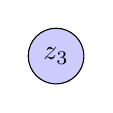
\begin{tikzpicture}
\node[draw, circle, fill=blue!20] (z3) {$ z_{3} $};
\end{tikzpicture}
\end{figure}
}
\only<2>{
\begin{figure}
\center
\begin{tikzpicture}
\node[draw, circle, fill=blue!20] (z3) {$ z_{3} $};
\node[draw, circle, fill=blue!20, below left =of z3] (z1) {$ z_{1} $};
\node[draw, circle, fill=blue!20, below right = of z3] (z2) {$ z_{2} $};
\draw[->, thick] (z3) -- (z1) node[midway, above, rotate=45] {$ \theta $};
\draw[->, thick] (z3) -- (z2) node[midway, above, rotate=315] {$ \theta $};
\end{tikzpicture}
\end{figure}
}
\only<3>{
\begin{figure}
\center
\begin{tikzpicture}
\node[draw, circle, fill=blue!20] (z3) {$ z_{3} $};

\node[draw, circle, fill=blue!20, below left =of z3] (z1) {$ z_{1} $};
\node[draw, circle, fill=blue!20, below right = of z3] (z2) {$ z_{2} $};

\node[draw, circle, fill=blue!20, below left= of z1] (in1) {$ \tilde{x}_{1} $};
\node[draw, circle, fill=blue!20, below left=of z2] (in2) {$ \tilde{x}_{2} $}; 
\node[draw, circle, fill=blue!20, below right= of z2] (in3) {$ \tilde{x}_{3} $};

\draw[->, thick] (z1) -- (in1) node[midway, above, rotate=45] {$ \theta $};
\draw[->, thick] (z1) -- (in2) node[midway, above, rotate=315] {$ \theta $};
\draw[->, thick] (z2) -- (in2) node[midway, above, rotate=45] {$ \theta $};
\draw[->, thick] (z2) -- (in3) node[midway, above, rotate=315] {$ \theta $};
\draw[->, thick] (z3) -- (z1) node[midway, above, rotate=45] {$ \theta $};
\draw[->, thick] (z3) -- (z2) node[midway, above, rotate=315] {$ \theta $};
\end{tikzpicture}
\end{figure}
}
\end{frame}

\begin{frame}[t]{Sleep Phase Update}
\hfill Compute $\log q(z|\tilde x, \lambda)$ and update $\lambda$
\begin{figure}
\center
\begin{tikzpicture}
\node[draw, circle, fill=orange] (z3) {$ z_{3} $};

\node[draw, circle, fill=orange, below left =of z3] (z1) {$ z_{1} $};
\node[draw, circle, fill=orange, below right = of z3] (z2) {$ z_{2} $};

\node[draw, rectangle, fill=gray, below left= of z1] (in1) {$ \tilde{x}_{1} $};
\node[draw, rectangle, fill=gray, below left=of z2] (in2) {$ \tilde{x}_{2} $}; 
\node[draw, rectangle, fill=gray, below right= of z2] (in3) {$ \tilde{x}_{3} $};

\draw[->, thick] (in1) -- (z1) node[midway, above, rotate=45] {$ \lambda $};
\draw[->, thick] (in2) -- (z1) node[midway, above, rotate=315] {$ \lambda $};
\draw[->, thick] (in2) -- (z2) node[midway, above, rotate=45] {$ \lambda $};
\draw[->, thick] (in3) -- (z2) node[midway, above, rotate=315] {$ \lambda $};
\draw[->, thick] (z1) -- (z3) node[midway, above, rotate=45] {$ \lambda $};
\draw[->, thick] (z2) -- (z3) node[midway, above, rotate=315] {$ \lambda $};
\end{tikzpicture}
\end{figure}
\end{frame}

\begin{frame}{Wake-sleep Algorithm}
\textbf{Advantages}
\begin{itemize}
\item Simple layer-wise updates
\item Amortised inference: all latent variables are inferred from the same weights $ \lambda $
\end{itemize}
\pause
\textbf{Drawbacks}
\begin{itemize}
\item Inference and generative networks are trained on different objectives
\item Inference weights $ \lambda $ are updated on fake data $ \tilde{x} $
\item Generative weights are bad initially, giving wrong signal to the updates of $ \lambda $
\end{itemize}
\end{frame}
